% Generated by paper/export_memory_diagnostics_tikz.py.
% Requires \usepackage{pgfplots} and \pgfplotsset{compat=1.18}.
% Input inside a subfigure; do not resizebox the result (fonts would shrink).
\begingroup
\definecolor{diagKeep}{HTML}{4C8C4A}
\definecolor{diagFifo}{HTML}{D55E00}
\definecolor{diagUnbounded}{HTML}{4D4D4D}
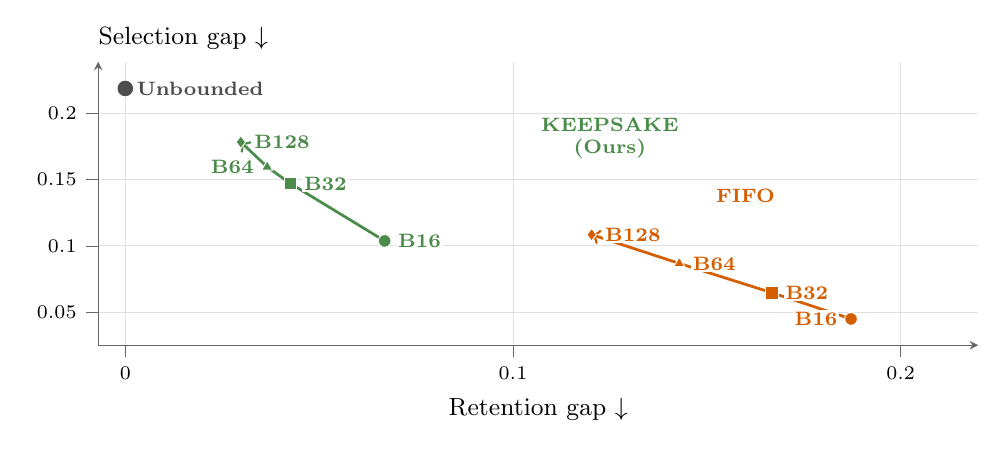
\begin{tikzpicture}
% Exact original 180-s / 13-trajectory rounded points, with RI omitted.
\begin{axis}[
  scale only axis, width=\dimexpr\linewidth-27pt\relax, height=36mm,
  xmin=-0.007, xmax=0.220, ymin=0.025, ymax=0.239,
  xtick={0,0.10,0.20}, ytick={0.05,0.10,0.15,0.20},
  scaled ticks=false,
  tick label style={font=\scriptsize,/pgf/number format/fixed,/pgf/number format/precision=2},
  label style={font=\small},
  xlabel={Retention gap $\downarrow$},
  axis lines=left, axis line style={black!60}, tick style={black!60},
  tick align=outside, grid=major, grid style={black!12,line width=0.25pt},
  clip=false, enlargelimits=false,
]
\node[anchor=south west,font=\small,inner sep=0pt]
  at (rel axis cs:0,1.04) {Selection gap $\downarrow$};
\addplot[diagFifo,line width=1pt,mark=none,->] coordinates {(0.1872,0.0448) (0.1668,0.0646) (0.1429,0.0867) (0.1203,0.1084)};
\addplot[only marks,diagFifo,mark=*,mark size=2.3pt,
  mark options={draw=white,line width=0.35pt,fill=diagFifo}] coordinates {(0.1872,0.0448)};
\node[anchor=east,font=\scriptsize\bfseries,text=diagFifo,
  inner sep=0.7pt,fill=white,xshift=-4pt]
  at (axis cs:0.1872,0.0448) {B16};
\addplot[only marks,diagFifo,mark=square*,mark size=2.3pt,
  mark options={draw=white,line width=0.35pt,fill=diagFifo}] coordinates {(0.1668,0.0646)};
\node[anchor=west,font=\scriptsize\bfseries,text=diagFifo,
  inner sep=0.7pt,fill=white,xshift=4pt]
  at (axis cs:0.1668,0.0646) {B32};
\addplot[only marks,diagFifo,mark=triangle*,mark size=2.3pt,
  mark options={draw=white,line width=0.35pt,fill=diagFifo}] coordinates {(0.1429,0.0867)};
\node[anchor=west,font=\scriptsize\bfseries,text=diagFifo,
  inner sep=0.7pt,fill=white,xshift=4pt]
  at (axis cs:0.1429,0.0867) {B64};
\addplot[only marks,diagFifo,mark=diamond*,mark size=2.3pt,
  mark options={draw=white,line width=0.35pt,fill=diagFifo}] coordinates {(0.1203,0.1084)};
\node[anchor=west,font=\scriptsize\bfseries,text=diagFifo,
  inner sep=0.7pt,fill=white,xshift=4pt]
  at (axis cs:0.1203,0.1084) {B128};
\addplot[diagKeep,line width=1pt,mark=none,->] coordinates {(0.0669,0.1037) (0.0426,0.1470) (0.0366,0.1596) (0.0298,0.1783)};
\addplot[only marks,diagKeep,mark=*,mark size=2.3pt,
  mark options={draw=white,line width=0.35pt,fill=diagKeep}] coordinates {(0.0669,0.1037)};
\node[anchor=west,font=\scriptsize\bfseries,text=diagKeep,
  inner sep=0.7pt,fill=white,xshift=4pt]
  at (axis cs:0.0669,0.1037) {B16};
\addplot[only marks,diagKeep,mark=square*,mark size=2.3pt,
  mark options={draw=white,line width=0.35pt,fill=diagKeep}] coordinates {(0.0426,0.1470)};
\node[anchor=west,font=\scriptsize\bfseries,text=diagKeep,
  inner sep=0.7pt,fill=white,xshift=4pt]
  at (axis cs:0.0426,0.1470) {B32};
\addplot[only marks,diagKeep,mark=triangle*,mark size=2.3pt,
  mark options={draw=white,line width=0.35pt,fill=diagKeep}] coordinates {(0.0366,0.1596)};
\node[anchor=east,font=\scriptsize\bfseries,text=diagKeep,
  inner sep=0.7pt,fill=white,xshift=-4pt]
  at (axis cs:0.0366,0.1596) {B64};
\addplot[only marks,diagKeep,mark=diamond*,mark size=2.3pt,
  mark options={draw=white,line width=0.35pt,fill=diagKeep}] coordinates {(0.0298,0.1783)};
\node[anchor=west,font=\scriptsize\bfseries,text=diagKeep,
  inner sep=0.7pt,fill=white,xshift=4pt]
  at (axis cs:0.0298,0.1783) {B128};
\addplot[only marks,diagUnbounded,mark=*,mark size=2.6pt]
  coordinates {(0,0.2188)};
\node[anchor=west,font=\scriptsize\bfseries,text=diagUnbounded,xshift=4pt,inner sep=0pt]
  at (axis cs:0,0.2188) {Unbounded};
\node[font=\scriptsize\bfseries,text=diagFifo,inner sep=1pt]
  at (axis cs:0.16,0.138) {FIFO};
\node[font=\scriptsize\bfseries,text=diagKeep,align=center,inner sep=1pt]
  at (axis cs:0.125,0.181) {KEEPSAKE\\(Ours)};
\end{axis}
\end{tikzpicture}
\endgroup
